\clearpage
%%=========================================
% Den litt rare section-formuleringen er for å en kortere header-tittel siden den er for lang ellers.
% \sectionmark{} inne i {section title as seen in paper ...} er for å få riktig header der en section begynner på en oddetallsside.
%
%   \section[section title as seen in TOC]{section title as seen in paper%
%       \sectionmark{section title as seen in header}}\sectionmark{section title as seen in header}
%
\section[Surface Analysis of Substrate A with Surface Pre-Growth Preparation]{Surface Analysis of Substrate A with Surface Pre-Growth Preparation%
    \sectionmark{Surface Analysis of Pre-Growth Substrate A}}\sectionmark{Surface Analysis of Pre-Growth Substrate A}\label{sec:subAb}

The dark field images taken of the surface of substrate A after etching show that the surface pre-growth preparation has left more particles on the surface than before, see Fig.~\ref{fig:subAa_om_df} and Fig.~\ref{fig:subAb_om_df}. The density of particles and features larger than \SI{0.5}{\micro\metre} has increased from \SI{\sim 4e2}{\centi\metre^{-2}} to \SI{\sim 1e3}{\centi\metre^{-2}} at the centre of the substrate.

\begin{figure}[htbp]
    \centering
    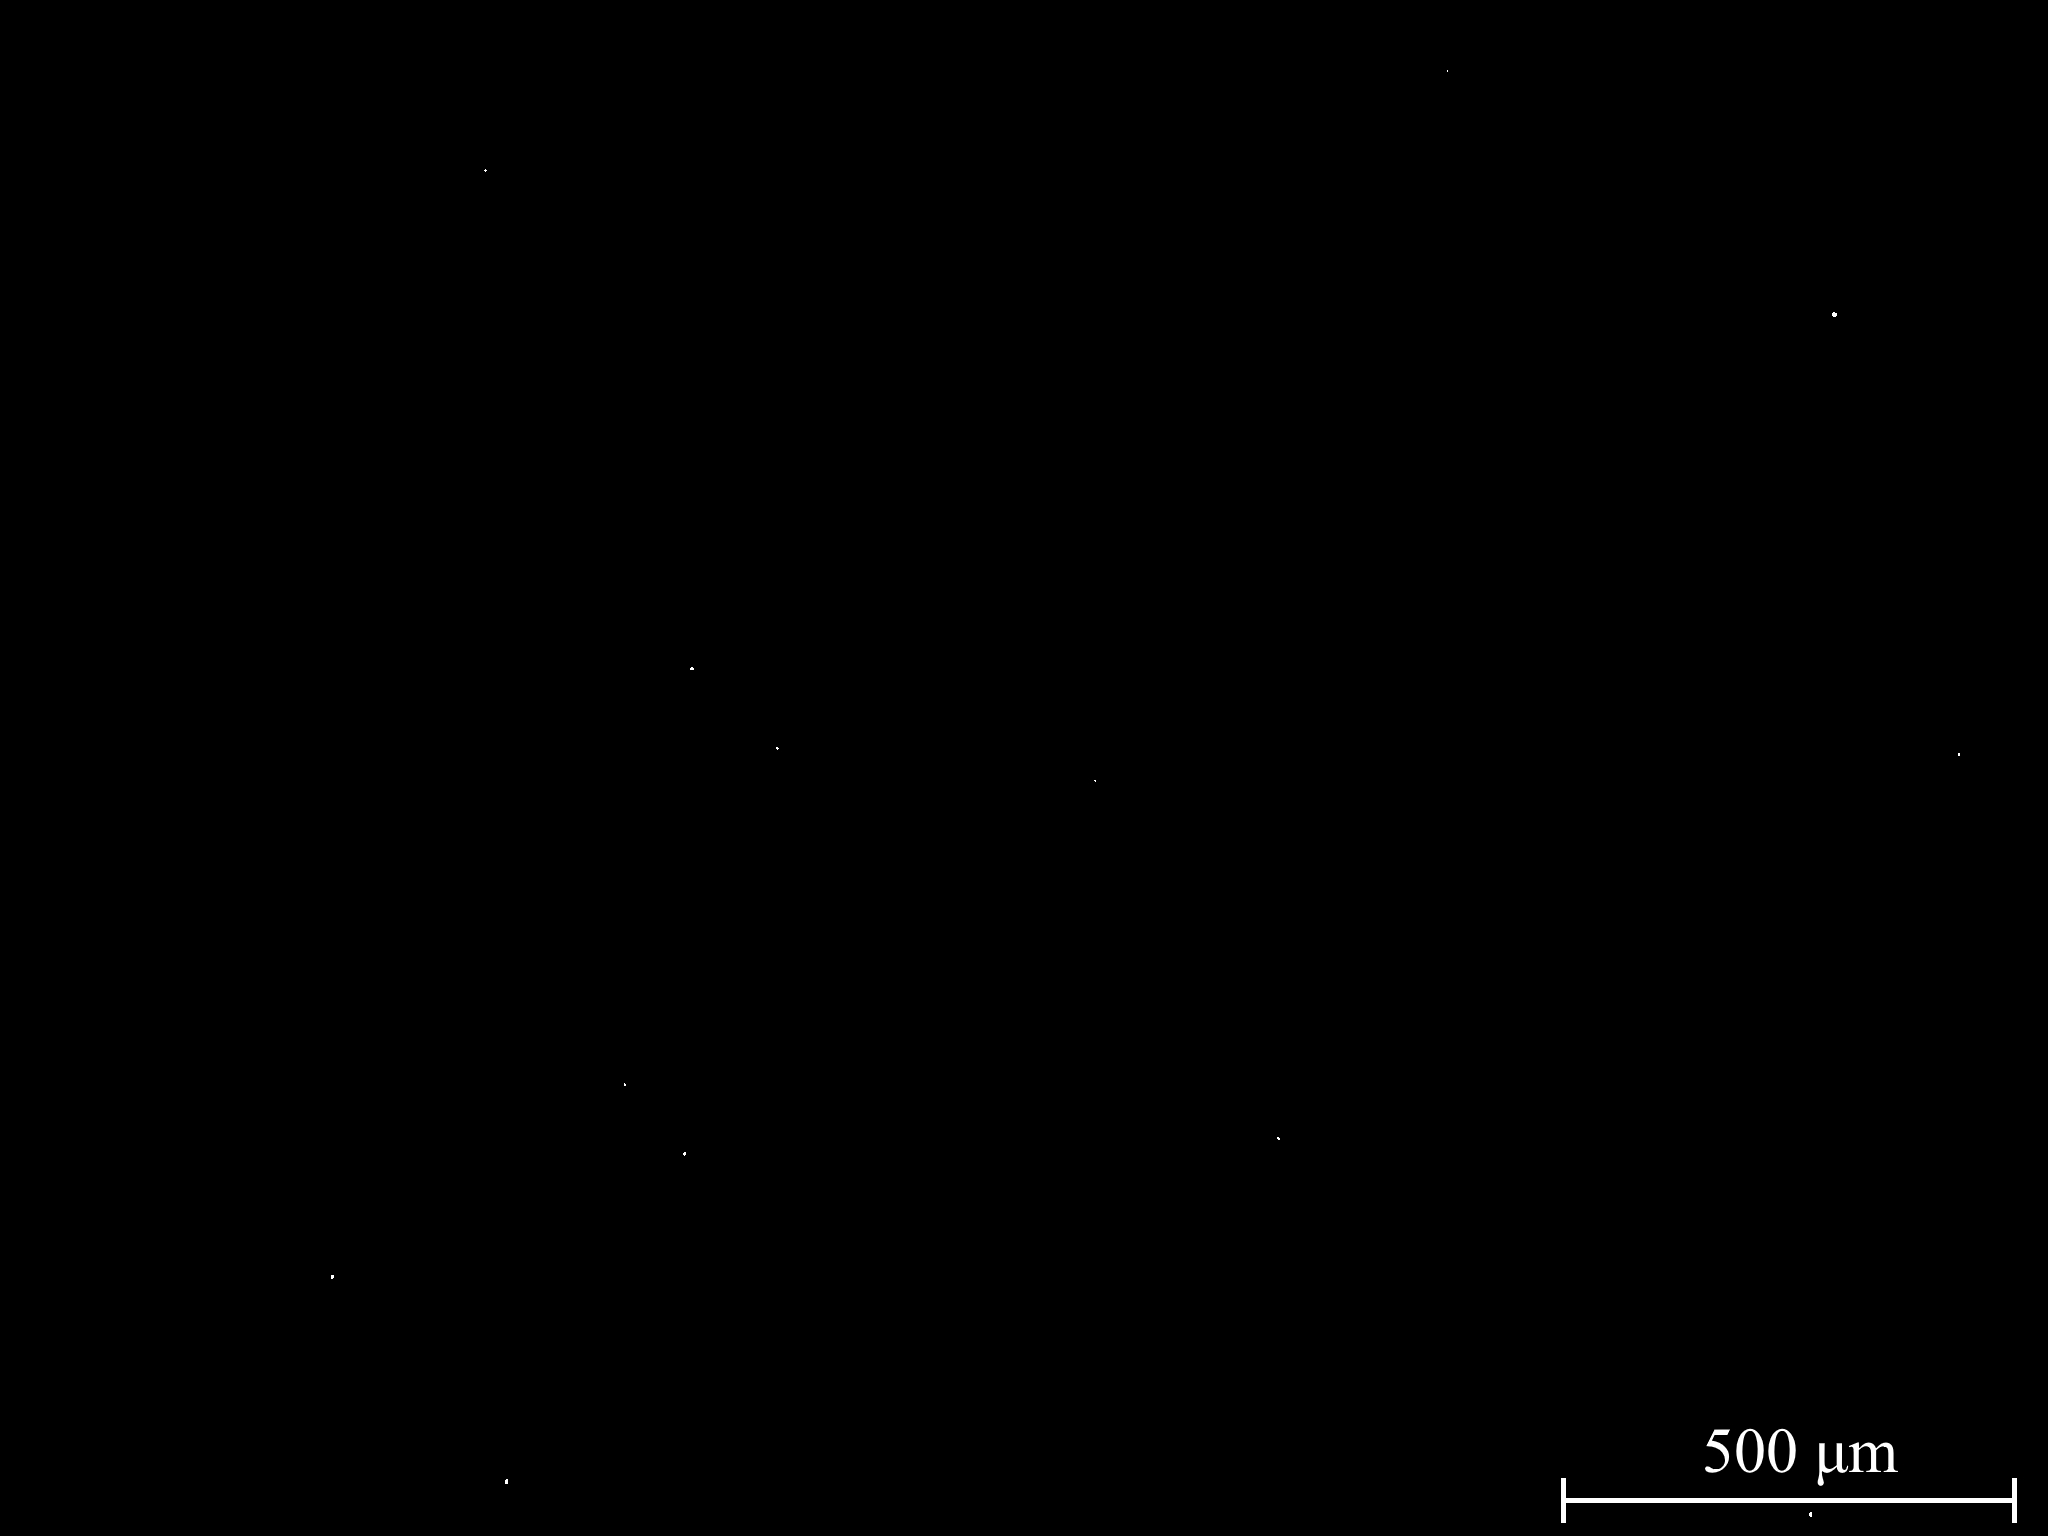
\includegraphics[width=0.8\linewidth]{subAb_om_df_n021.jpg}
    \caption[Dark field optical microscopy image of substrate A with surface pre-growth preparation.]{Dark field optical microscopy image of substrate A with surface pre-growth preparation taken near the centre of the substrate at a magnification of $5\times$.}\label{fig:subAb_om_df}
\end{figure}

\Ac{sem} shows the surface at a higher magnification and it reveals that there are much smaller particles distributed over the surface as well. Fig.~\ref{fig:subAb_sem_typical_centre} shows a typical image of an area near the centre of the substrate. Here the particle density is  \SI{\sim 2e+06}{\particle\centi\metre^{-2}}. The highest observed density of particles is counted near the upper edge to be \SI{3e+07}{\particle\centi\metre^{-2}}, see Fig.~\ref{fig:subAb_sem_typical_edge}.

\begin{figure}[htbp]
    \begin{subfigure}[t]{0.49\textwidth}
        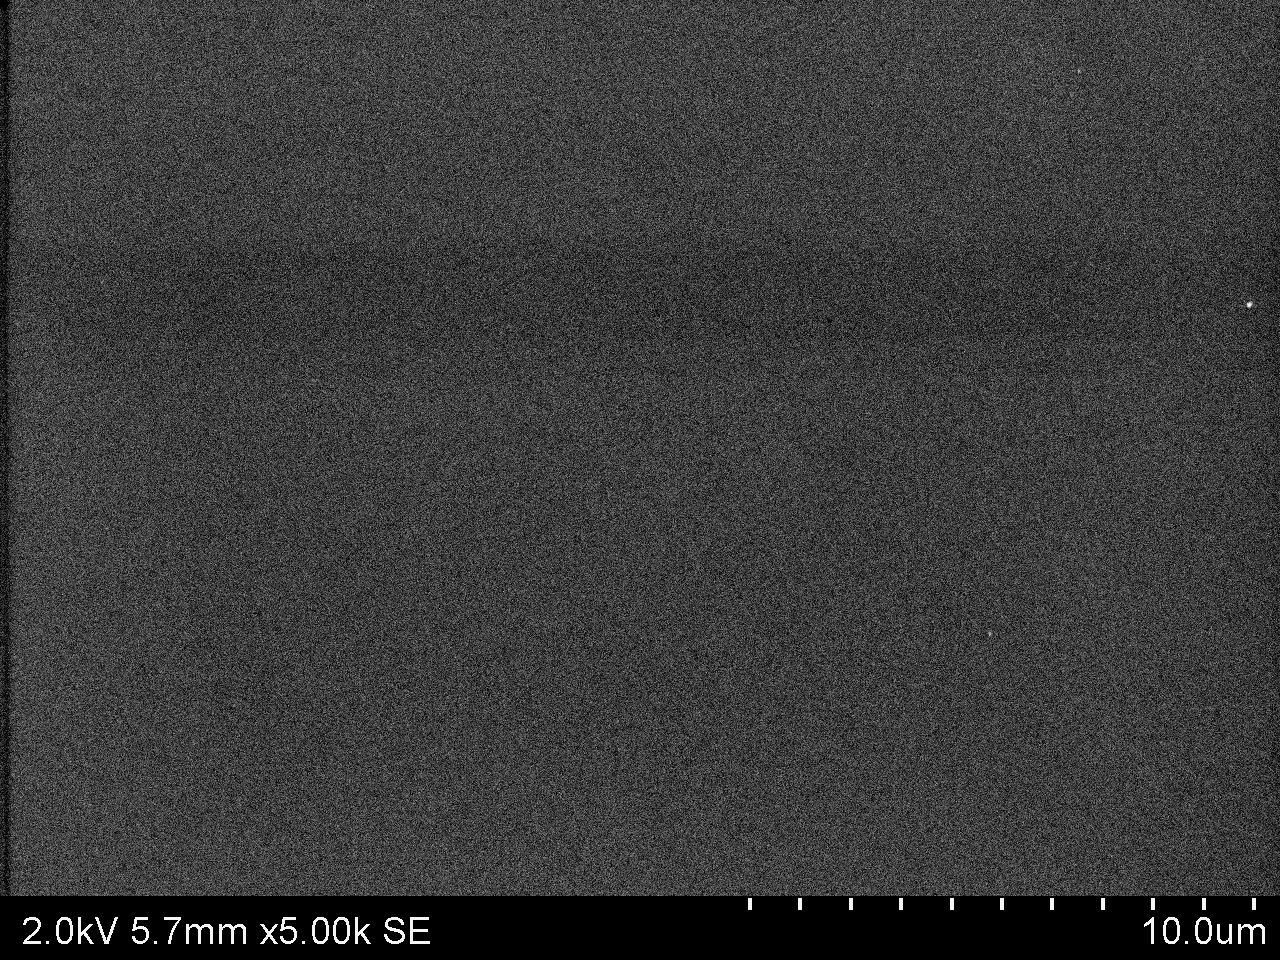
\includegraphics[width=\linewidth]{subAb_sem_02b_m008.png}
        \caption{Near the centre.}\label{fig:subAb_sem_typical_centre}
    \end{subfigure}%
    \hfill
    \begin{subfigure}[t]{0.49\textwidth}
        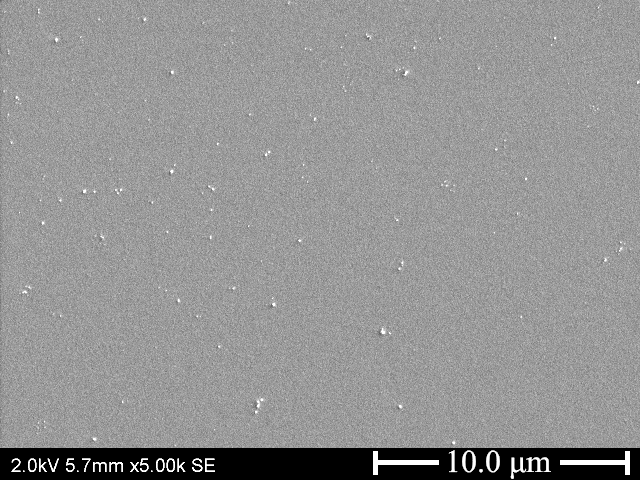
\includegraphics[width=\linewidth]{subAb_sem_02a_m004.png}
        \caption{Near the upper edge.}\label{fig:subAb_sem_typical_edge}
    \end{subfigure}%
    \caption[\Ac{sem} images of typical areas on substrate A with surface pre-growth preparation.]{\Acf{sem} images of a typical area near the centre and an area with a high density of particles near the edge of substrate A after surface pre-growth preparation taken at a magnification of $5000\times$.}\label{fig:subAb_sem_typical}
\end{figure}

%%=========================================
\subsection{Particles}
Four different types of particles are observed on the surface of substrate A after surface pre-growth preparation, see Fig.~\ref{fig:subAb_sem_w_eds}. They will be described and identified in the following.

\begin{figure}
    \centering
    \begin{subfigure}[t]{\textwidth}
          \begin{minipage}[t]{0.49\linewidth}
            \centering
            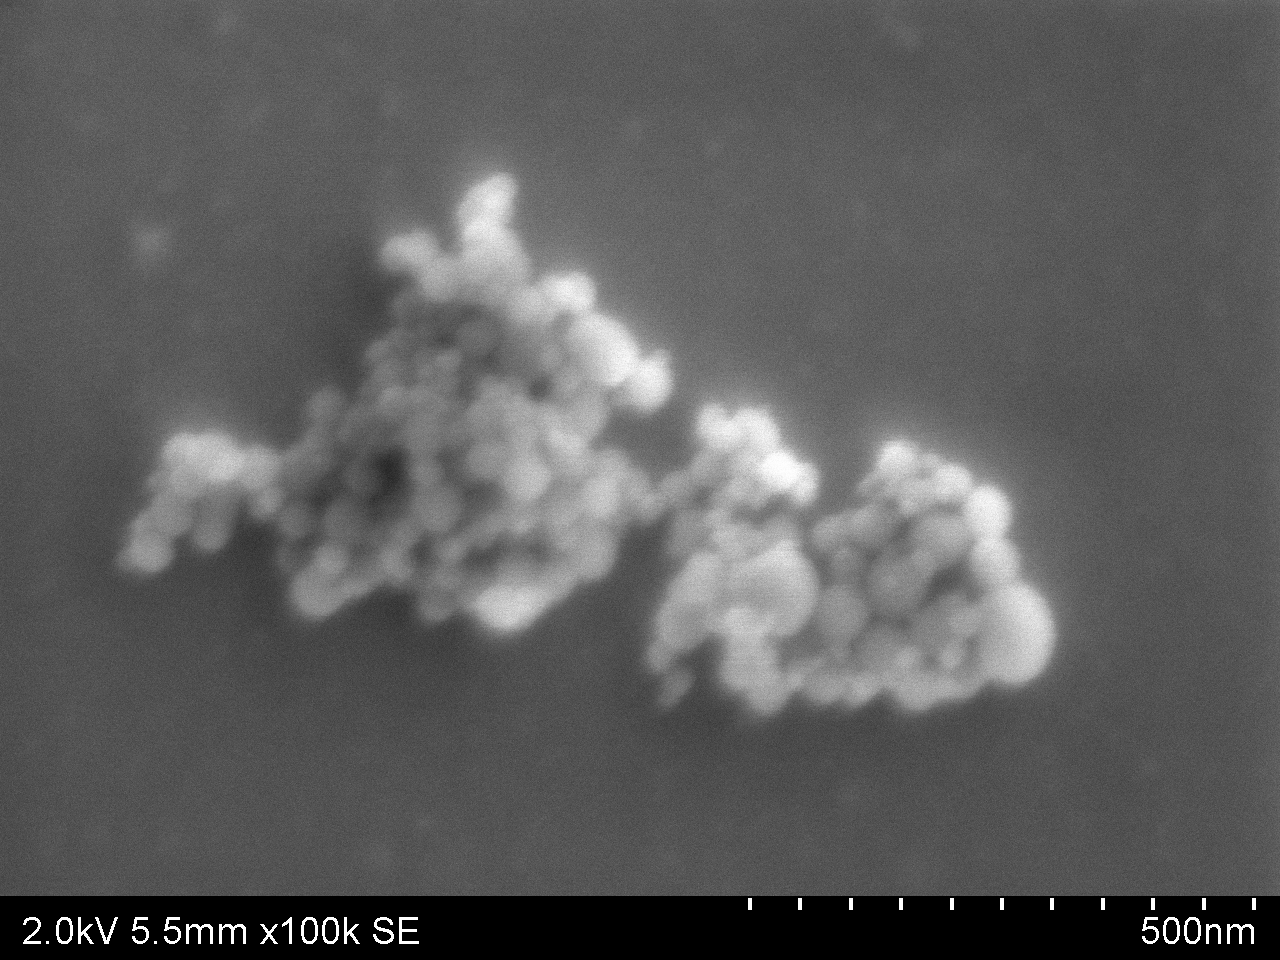
\includegraphics[width=\linewidth]{subAb_sem_03_m004.png}
          \end{minipage}
          \hspace{0.02\linewidth}
          \begin{minipage}[t]{0.49\linewidth}
            \centering
            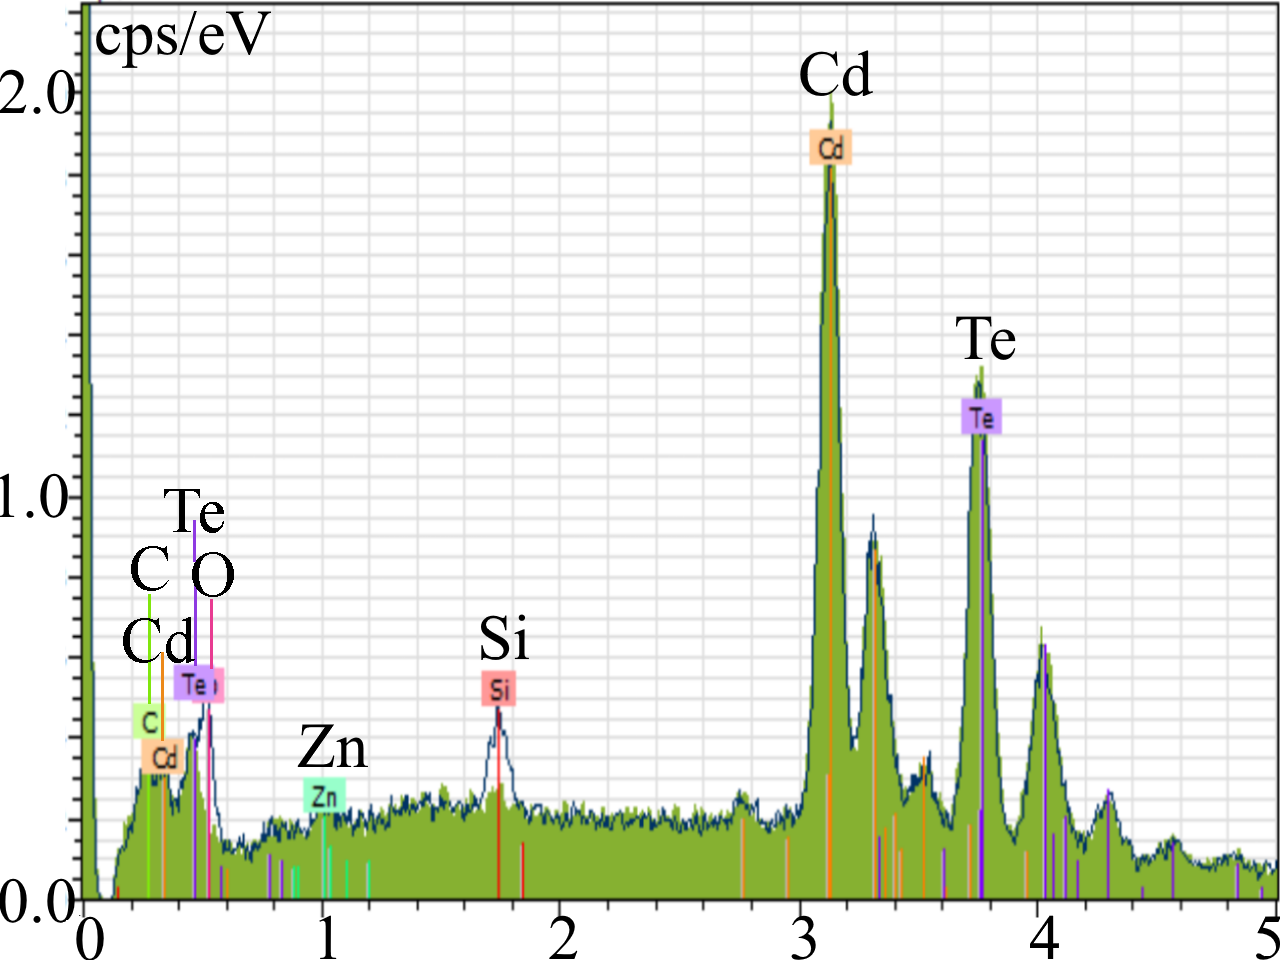
\includegraphics[width=\linewidth]{subAb_eds_03_m004.png}
          \end{minipage}
        \caption{Silica (\ce{SiO2}) polishing grit agglomeration.}\label{fig:subAb_silica}
    \end{subfigure}
    \par\bigskip
    \begin{subfigure}[t]{\textwidth}
          \begin{minipage}[t]{0.49\linewidth}
            \centering
            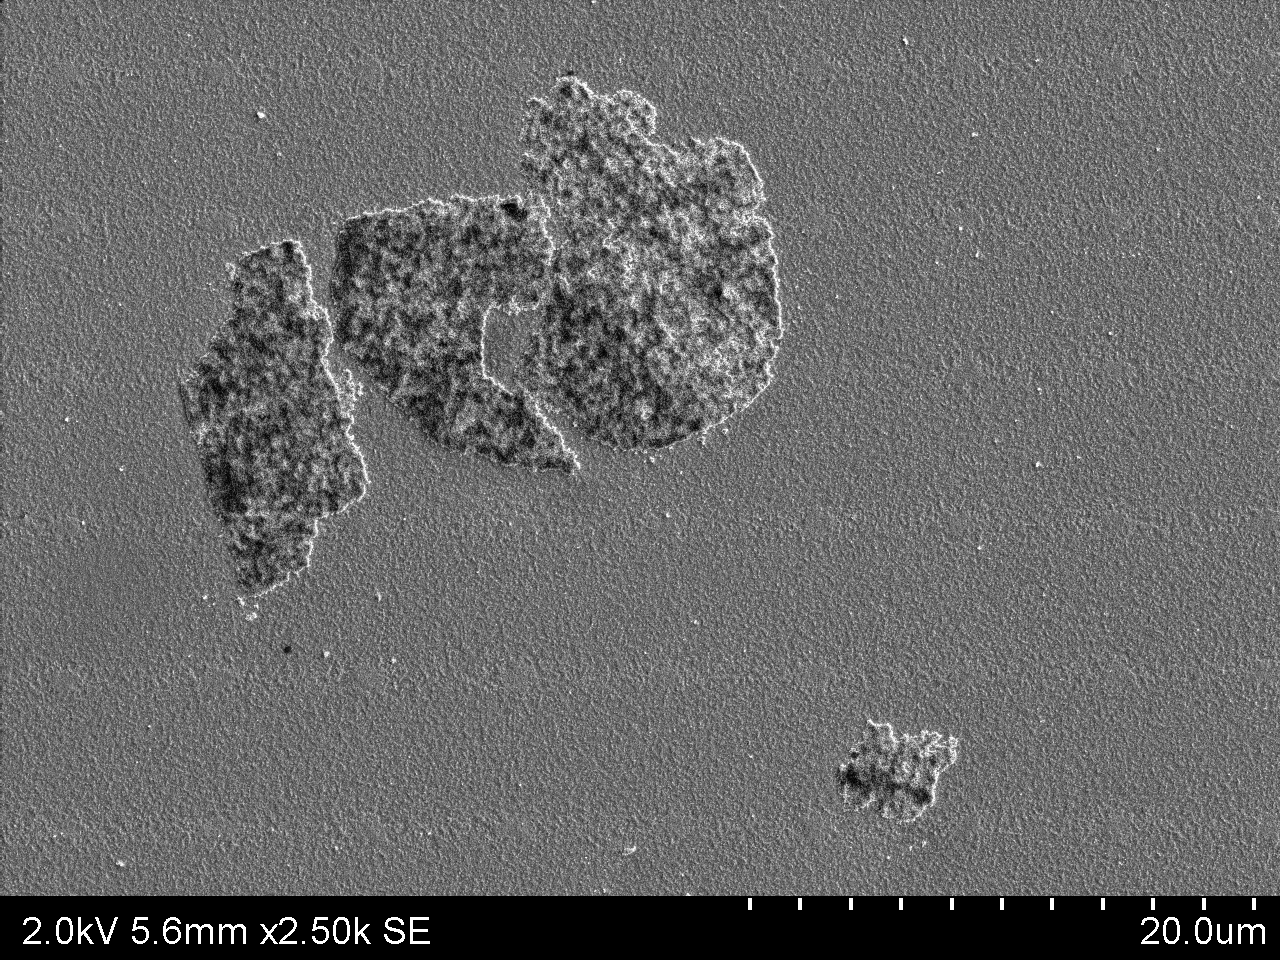
\includegraphics[width=\linewidth]{subAb_sem_03_m005.png}
          \end{minipage}
          \hspace{0.02\linewidth}
          \begin{minipage}[t]{0.49\linewidth}
            \centering
            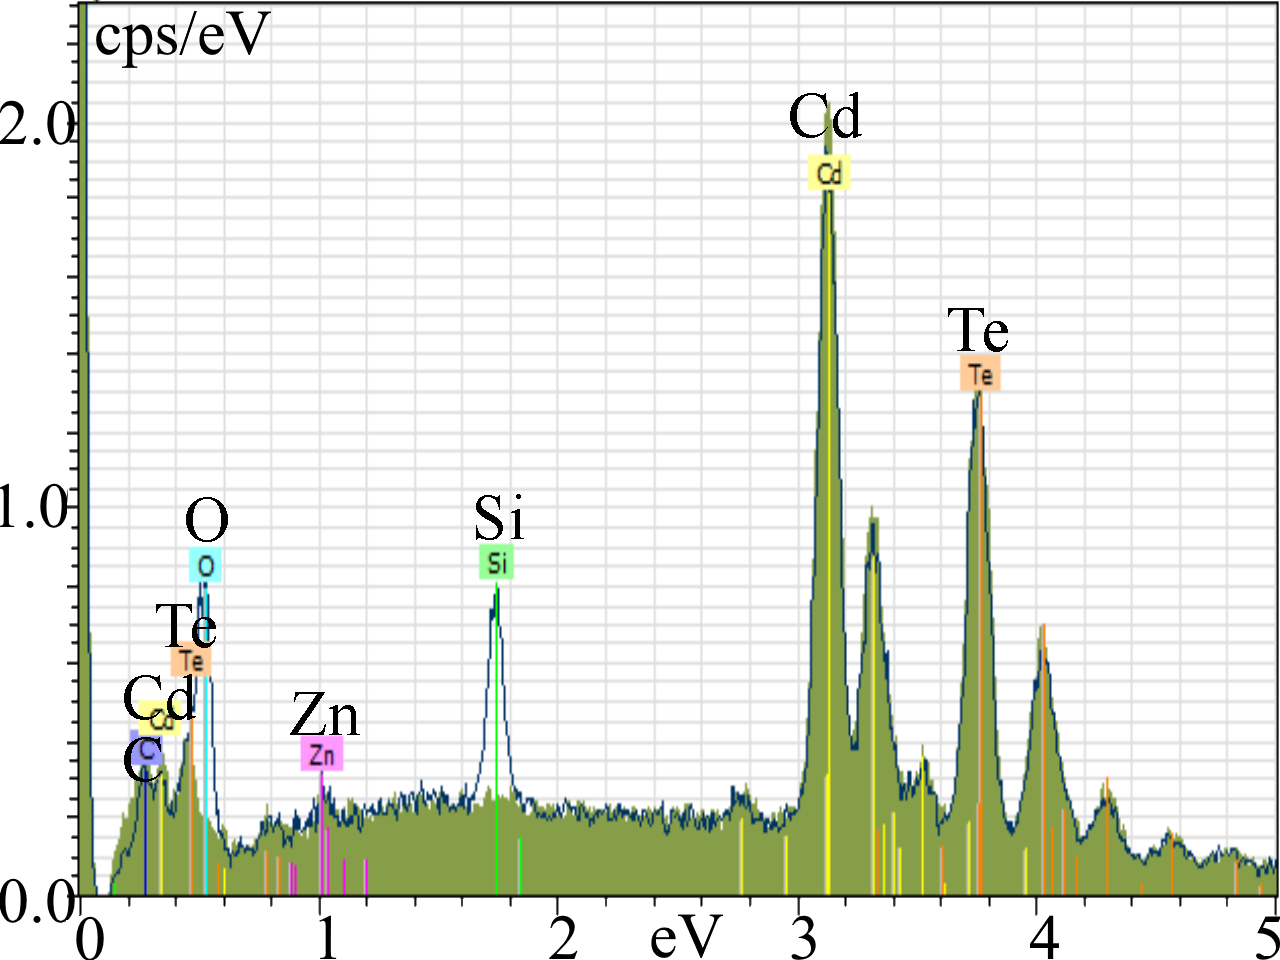
\includegraphics[width=\linewidth]{subAb_eds_03_m005.png}
          \end{minipage}
        \caption{Silica (\ce{SiO2}) particles.}\label{fig:subAb_silica2}
    \end{subfigure}
    \par\bigskip
    \begin{subfigure}[t]{\textwidth}
          \begin{minipage}[t]{0.49\linewidth}
            \centering
            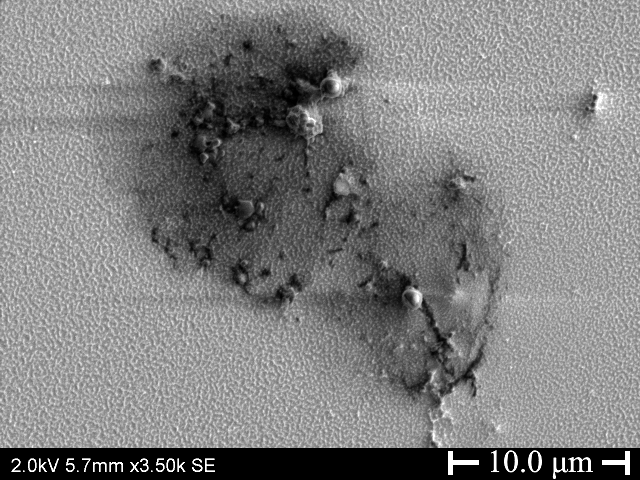
\includegraphics[width=\linewidth]{subAb_sem_03_m011.png}
          \end{minipage}
          \hspace{0.02\linewidth}
          \begin{minipage}[t]{0.49\linewidth}
            \centering
            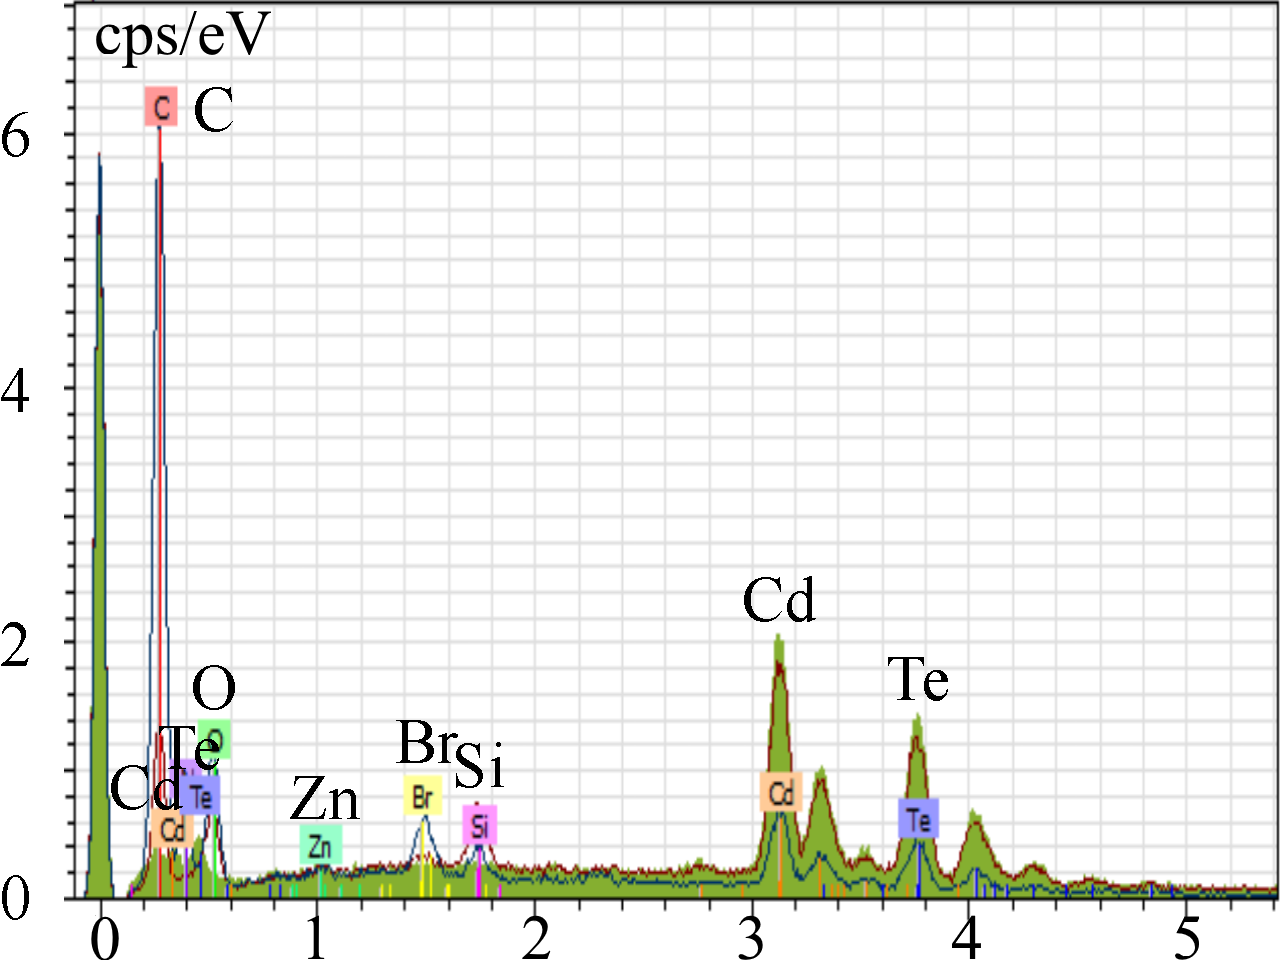
\includegraphics[width=\linewidth]{subAb_eds_03_m011.png}
          \end{minipage}
        \caption{Stain consisting of bromine, carbon, and oxygen.}\label{fig:subAb_br-stain}
    \end{subfigure}
    \caption[\Ac{sem} images and \ac{eds} spectra of particles found on substrate A after surface pre-growth preparation.]{High resolution \acf{sem} images of particles found on substrate A after surface pre-growth preparation and the corresponding \acf{eds} spectra of the particles. The blue line represents the \ac{eds} spectrum of the particle, while the filled green represents the \ac{eds} spectrum of the underlying substrate.}\label{fig:subAb_sem_w_eds}
\end{figure}

\begin{figure}[htbp]
\ContinuedFloat
    \centering
    \begin{subfigure}[t]{\textwidth}
          \begin{minipage}[t]{0.49\linewidth}
            \centering
            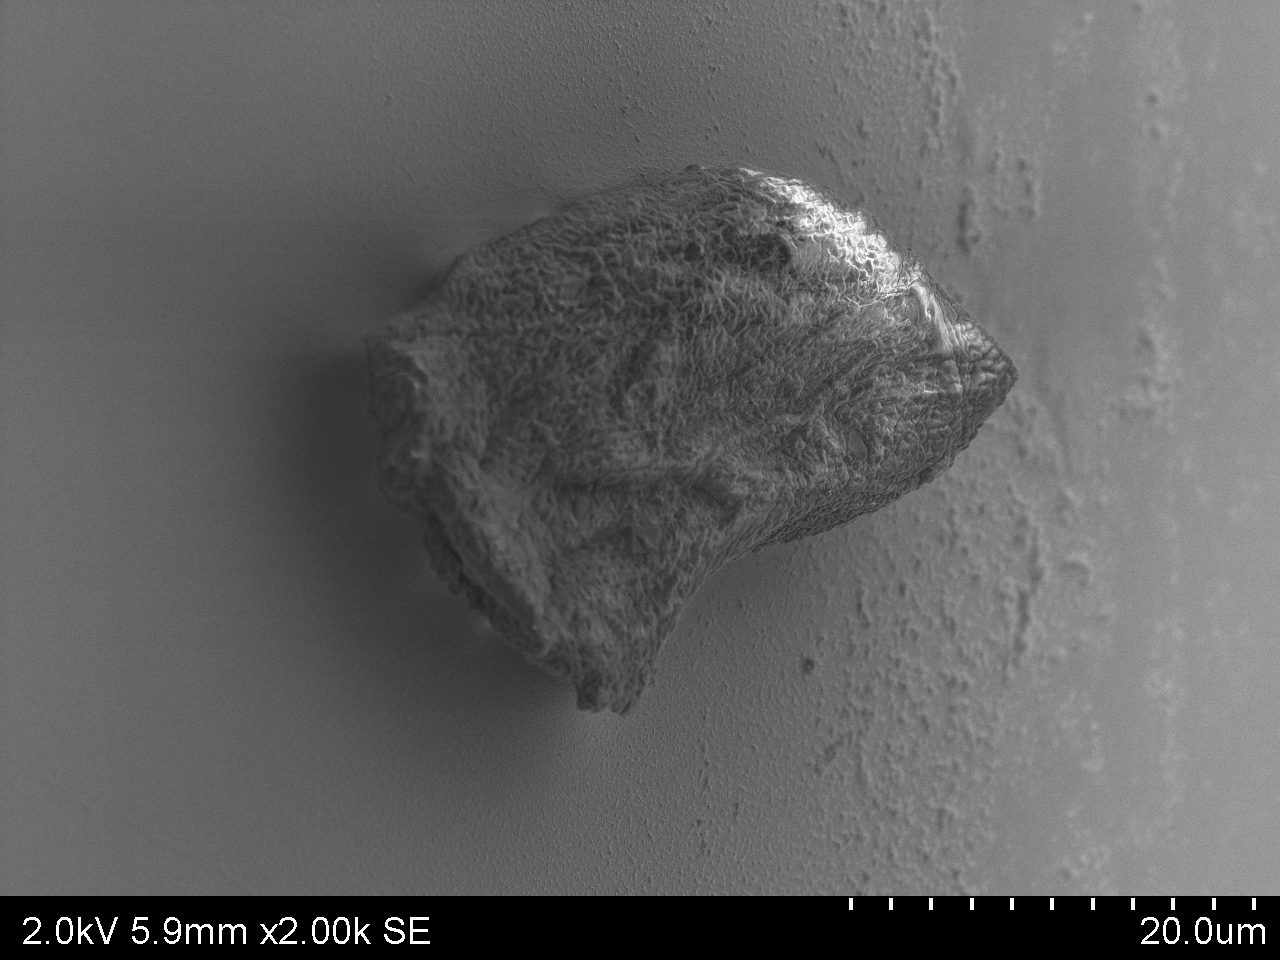
\includegraphics[width=\linewidth]{subAb_sem_03_m013.png}
          \end{minipage}
          \hspace{0.02\linewidth}
          \begin{minipage}[t]{0.49\linewidth}
            \centering
            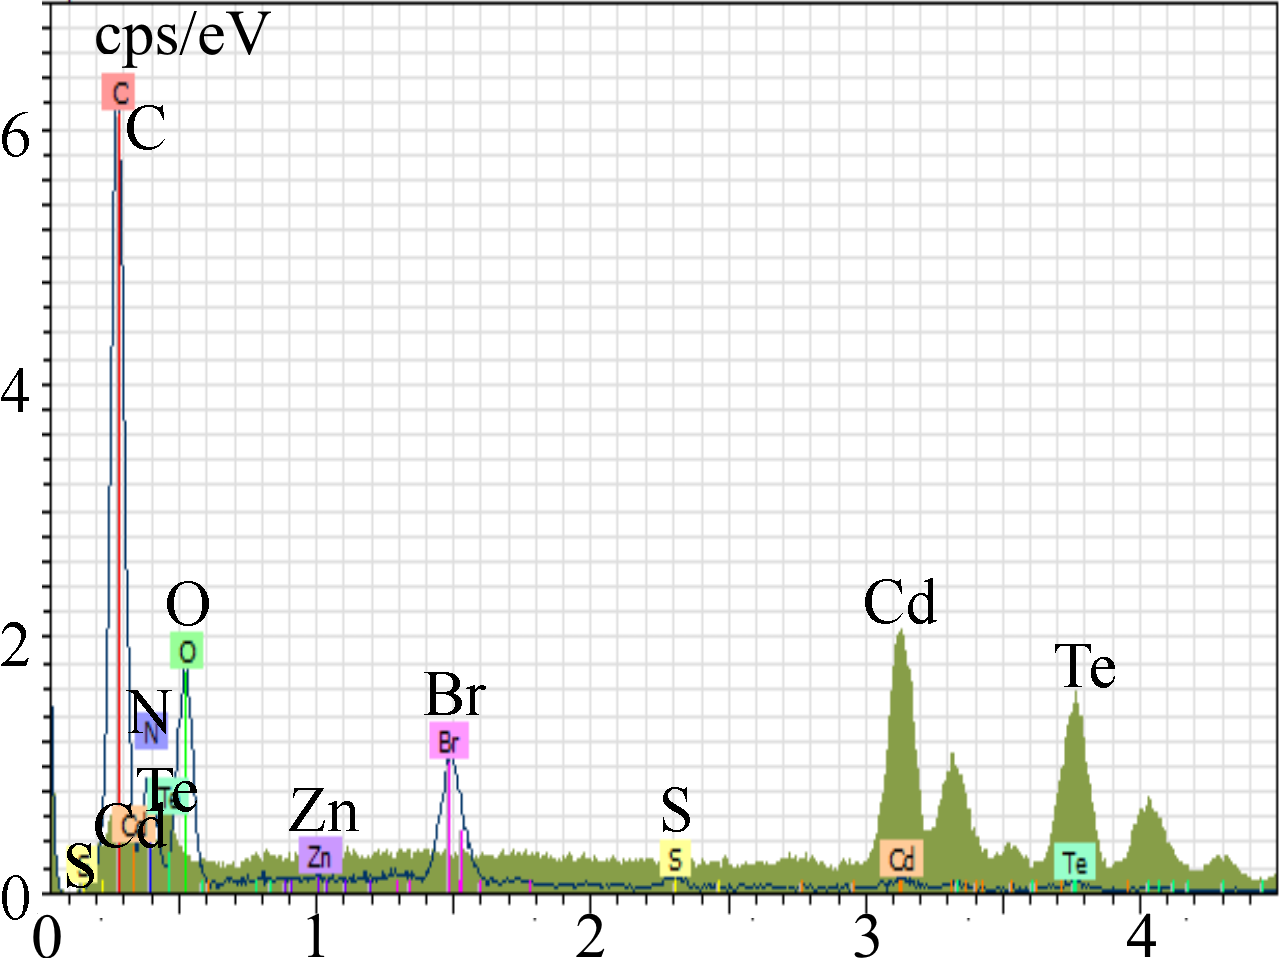
\includegraphics[width=\linewidth]{subAb_eds_03_m013.png}
          \end{minipage}
        \caption{Particle consisting of bromine, carbon, and oxygen.}\label{fig:subAb_br-particle}
    \end{subfigure}
    \captionsetup{list=no}
    \caption{\emph{(continued)}}
\end{figure}

As before the preparation, silica polishing grit is found on the surface of the substrate, see Fig.~\ref{fig:subAb_silica}. However, the grit density is higher and there are larger agglomerations of grit. The polishing grit could originate from the edges of the as-received substrate and have been distributed over the surface during preparation by the etch solution.

The silica polishing grit observed in \ac{sem} are found all over the surface. The particle density was found to be between \SI{2e+06}{\particle\centi\metre^{-2}} and \SI{3e+07}{\particle\centi\metre^{-2}}. The mean particle density was \SI{7e+06}{\particle\centi\metre^{-2}} with a standard deviation of \SI{7e+06}{\particle\centi\metre^{-2}}. A graphical representation of the particle density at different locations on substrate A can be seen in Fig.~\ref{fig:subAb_densityData}. There is a tendency of higher density towards the upper right and lower left corners.

\begin{figure}[htbp]
    \centering
    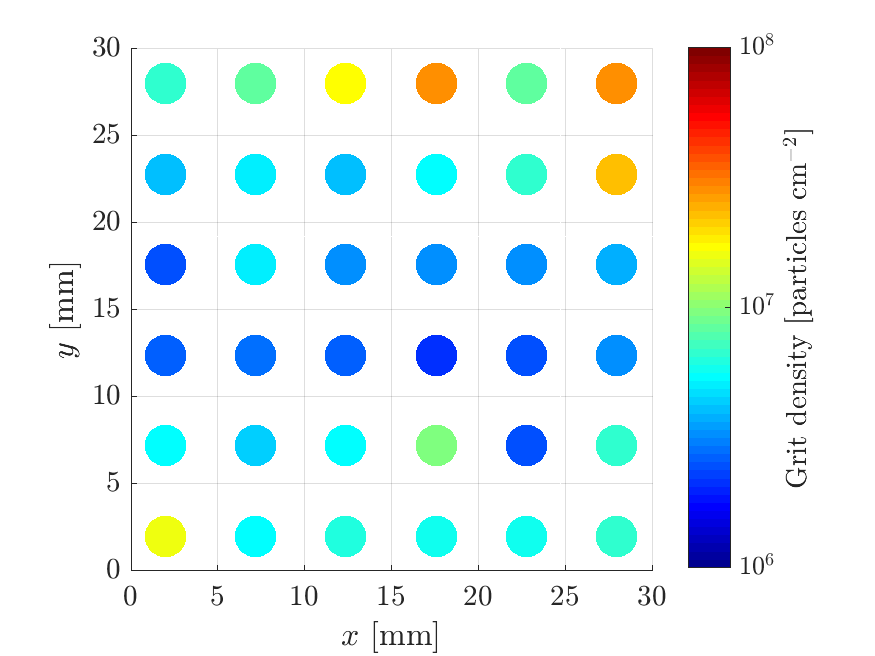
\includegraphics[width=0.8\linewidth]{subAb_densityData.png}
    \caption[Map of the polishing grit density on substrate A after surface pre-growth preparation.]{A map of the polishing grit density at 36 different locations on the $\SI{30}{\milli\metre}\times\SI{30}{\milli\metre}$ substrate A after surface pre-growth preparation. The polishing grit density was observed to vary between \SI{2e+06}{\particle\centi\metre^{-2}} and \SI{3e+07}{\particle\centi\metre^{-2}}.}
    \label{fig:subAb_densityData}
\end{figure}

Fig.~\ref{fig:subAb_silica2} shows four particles ranging from \SI{4}{\micro\metre} to \SI{15}{\micro\metre} in size. These particles consists of \ce{SiO2}. When looking at the particles at higher magnification, see Fig.~\ref{fig:subAb_silica2_magnified}, it appears that they are made up of smaller, circular particles with a diameter of \SIrange{50}{100}{\nano\metre}. Possibly silica polishing grit that have accumulated to a larger structure. These structures are mainly observed near the edges of the substrate.

\begin{figure}
    \centering
    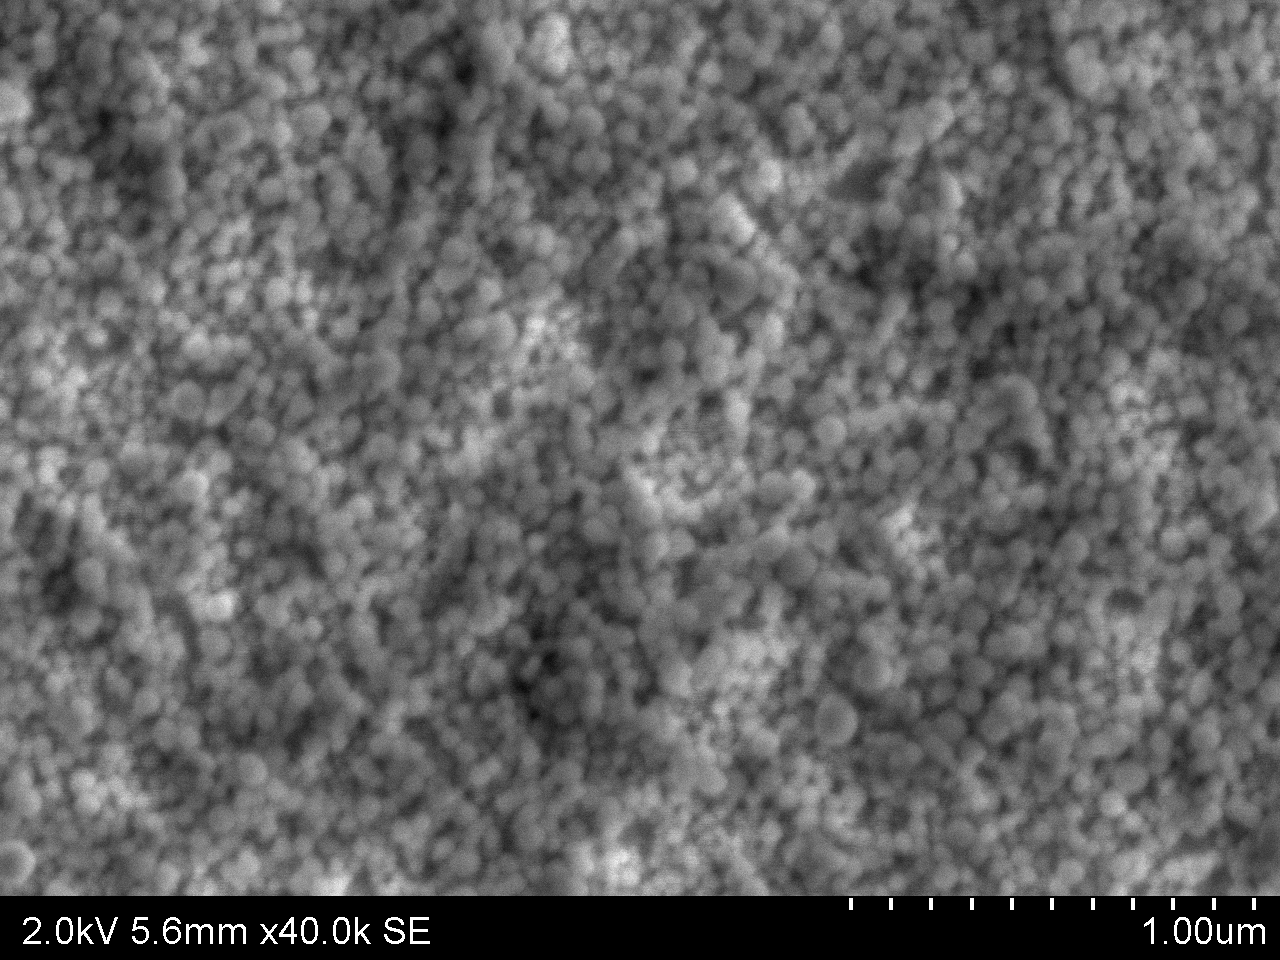
\includegraphics[width=0.8\linewidth]{subAb_sem_03_m006.png}
    \caption[\Ac{sem} image of silica flake.]{\Acf{sem} image of flake consisting of silica (\ce{SiO2}).}\label{fig:subAb_silica2_magnified}
\end{figure}

Fig.~\ref{fig:subAb_br-stain} shows a stain that consists of bromine, carbon, and oxygen. This type of stain is observed mainly near the edges of substrate A. The stains are typically \SI{\sim10}{\micro\metre} long. Another type of particle showing the same composition in the \ac{eds} spectrum as the stain is also found around the edges of the substrate, see Fig.~\ref{fig:subAb_br-particle}. This particle is typically \SIrange{20}{30}{\micro\metre} long.

%%=========================================
%\section{AFM Study of Etched Substrate A}
\subsection{Surface Roughness}

\begin{figure}[htbp]
    \centering
    \begin{subfigure}[t]{\linewidth}
        \centering
        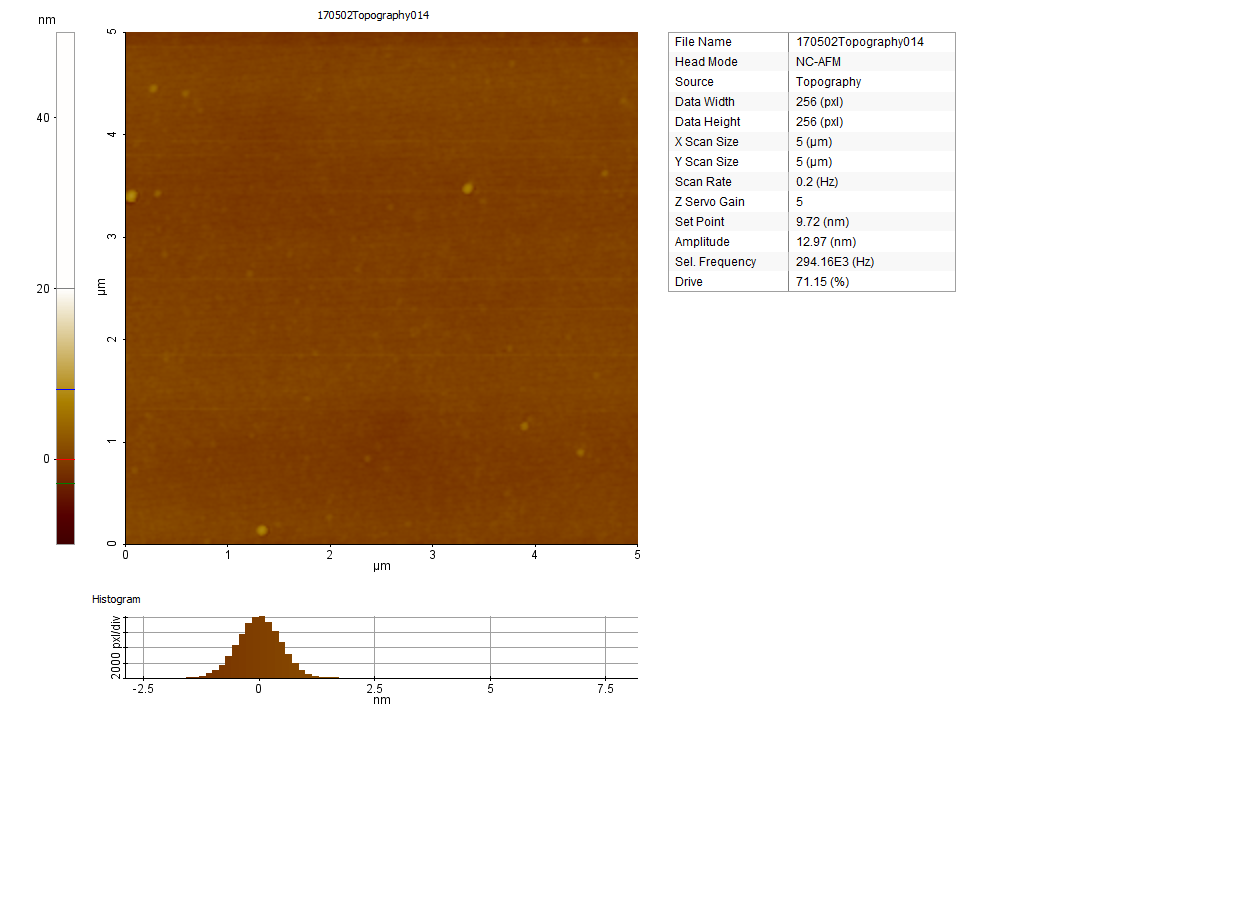
\includegraphics[width=0.5\linewidth,trim={0cm 12cm 21cm 0cm},clip]{170502Topography014_centre.png}
        \caption{Near centre, \ac{rms} roughness \SI{0.51}{\nano\metre}.} %\SI{0.85}{\nano\metre}
    \end{subfigure}%
    \par\bigskip
    \begin{subfigure}[t]{\linewidth}
        \centering
        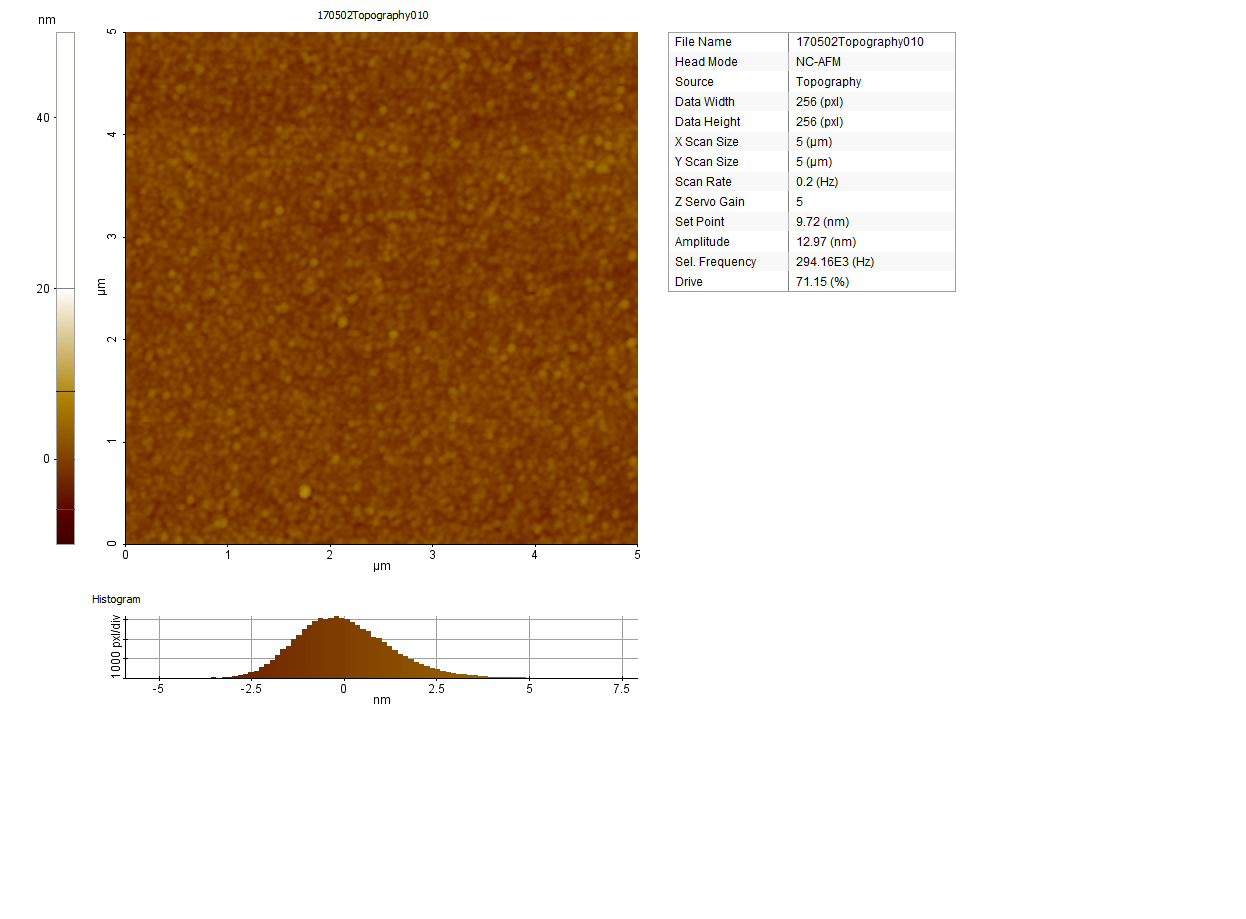
\includegraphics[width=0.5\linewidth,trim={0cm 12cm 21cm 0cm},clip]{170502Topography010_upperedge.png}
        \caption{Near upper edge, \ac{rms} roughness \SI{1.3}{\nano\metre}.} %\SI{0.77}{\nano\metre}}
    \end{subfigure}%
    \par\bigskip
    \begin{subfigure}[t]{\linewidth}
        \centering
        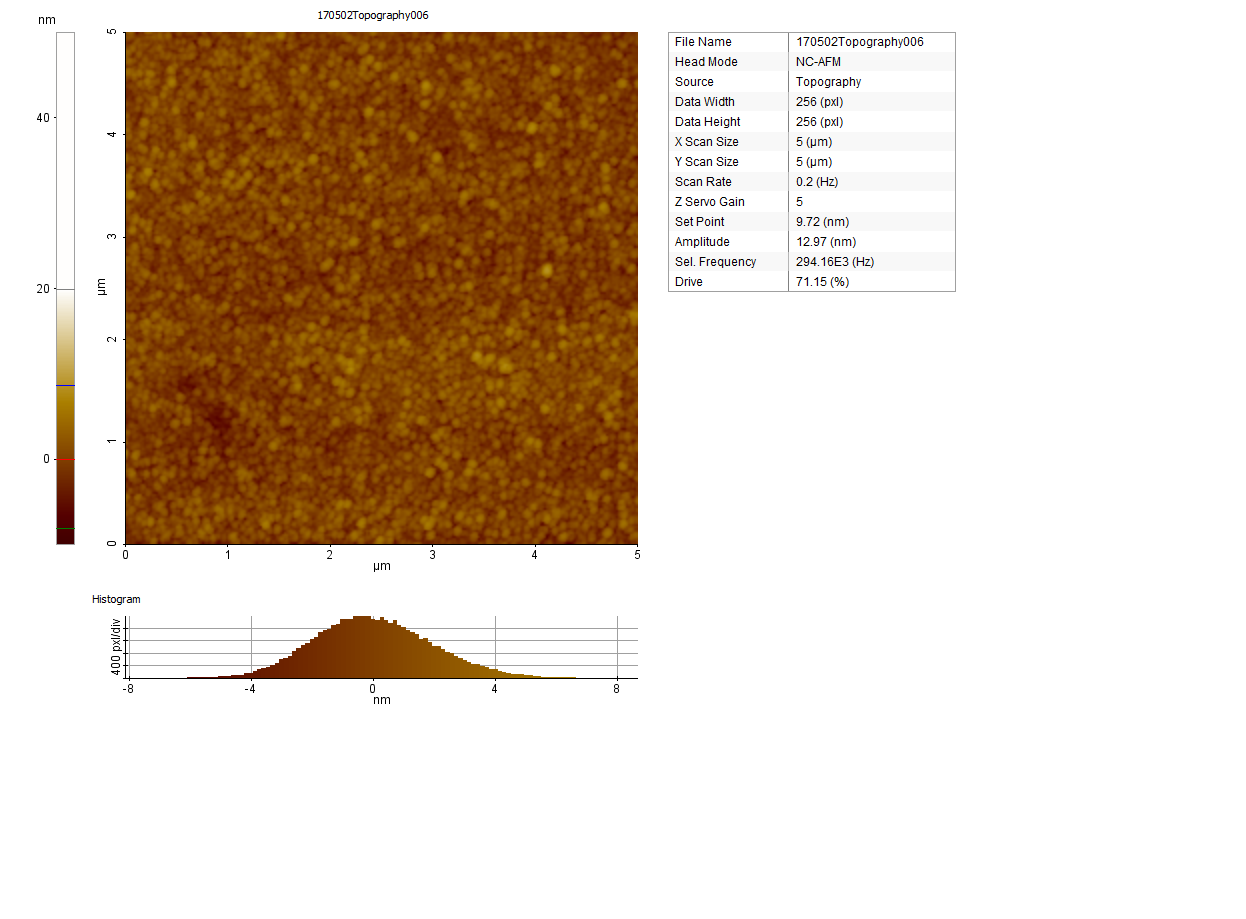
\includegraphics[width=0.5\linewidth,trim={0cm 12cm 21cm 0cm},clip]{170502Topography006_upperleftcorner.png}
        \caption{Near upper left corner, \ac{rms} roughness \SI{1.9}{\nano\metre}.}%\SI{1,04}{\nano\metre}
    \end{subfigure}%
    \caption[\Ac{afm} of substrate A with surface pre-growth preparation.]{\Acf{afm} measurements of substrate A with surface pre-growth preparation. Images of a $\SI{5}{\micro\metre}\times\SI{5}{\micro\metre}$ area are taken at the centre, edge, and corner of the substrate.}\label{fig:afm_subAb}
\end{figure} % AFM, substrate A, with surface pre-growth preparation.

%%=========================================
\subsection{Impurity Analysis}

\begin{table}[htbp]
    \centering
    \caption[\Ac{eds} impurity analysis of substrate A with surface pre-growth preparation.]{Results of the \acf{eds} impurity analysis at three different locations on the $30\times30$ \SI{}{\milli\metre^2} (111)B \ac{czt} substrate A with surface pre-growth preparation (atomic concentration \%). The X-ray signal is acquired from a $\SI{1270}{}\times\SI{890}{\micro\metre^2}$ area at a magnification of 100$\times$ near the upper left corner, upper edge, and centre.}\label{tab:subAb_eds_analysis}
   \begin{tabu} to 1.0\textwidth { X[1.85, r] X[1.125,c] X[1.125,c] X[1.125,c] X[1.125,c] X[1.125,c] X[1.125,c] X[1.125,c] } % X[1,c] X[1,c]
        \hline
            & \textbf{\ce{Te}} (at.\%) & \textbf{\ce{Cd}} (at.\%) & \textbf{\ce{Zn}} (at.\%) & \textbf{\ce{Al} } (at.\%) & \textbf{\ce{Si}} (at.\%) & \textbf{\ce{C}} (at.\%) & \textbf{\ce{O}} (at.\%) \\ % \textbf{$X$} (\SI{}{\milli\metre}) &  \textbf{$Y$} (\SI{}{\milli\metre})
        \hline
        Near corner & \SI{45.18}{} & \SI{44.79}{} & \SI{1.70}{} & \SI{0.56}{} & \SI{0.63}{} & \SI{6.45}{} & \SI{0.70}{} \\ % \SI{1.0}{}  & \SI{29.0}{}
        Near edge & \SI{45.41}{} & \SI{45.08}{} & \SI{1.72}{} & \SI{0.25}{} & \SI{0.60}{} & \SI{6.01}{} & \SI{0.95}{} \\ % \SI{15.0}{} & \SI{29.0}{} 
        Near centre & \SI{45.42}{} & \SI{44.95}{} & \SI{1.84}{} & \SI{0.22}{} & \SI{0.54}{} & \SI{6.05}{} & \SI{0.97}{} \\ % \SI{15.0}{} & \SI{15.0}{}
        \hline
    \end{tabu}
\end{table}
%%=========================================

